\frame
{
  \frametitle{Matrix Factorization Approach}

\begin{center}
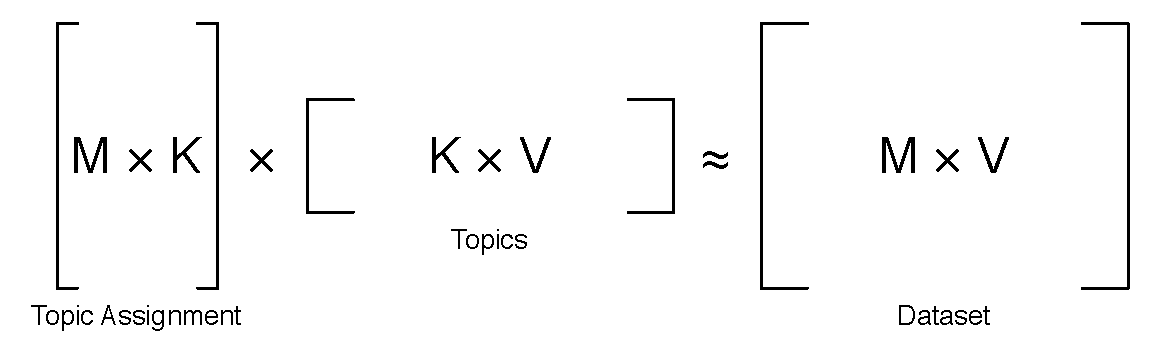
\includegraphics[width=0.9\linewidth]{topic_models/factorization.pdf}
\end{center}

\begin{columns}
\column{.5\textwidth}
\begin{block}{}
	\begin{itemize}
		\item[K] Number of topics
		\item[M] Number of documents
		\item[V] Size of vocabulary
	\end{itemize}
\end{block}
\column{.5\textwidth}
\pause
\begin{itemize}
\item If you use singular value decomposition (SVD), this technique is called latent semantic analysis.
\item Popular in information retrieval.
\end{itemize}
\end{columns}

}

\begin{frame}

\frametitle{Alternative: Generative Model}

\begin{itemize}
  \item How your data came to be
  \item Sequence of Probabilistic Steps
  \item Posterior Inference
\end{itemize}

\end{frame}

\begin{frame}
	\frametitle{Multinomial Distribution}

	\begin{itemize}
		\item Distribution over discrete outcomes
		\item Represented by non-negative vector that sums to one
		\item Picture representation
	\begin{center}
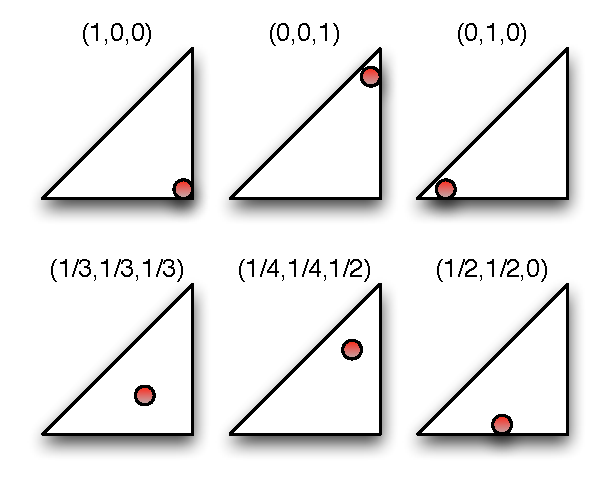
\includegraphics[width=0.4\linewidth]{topic_models/multinomial}
	\end{center}
		\pause
		\item Come from a Dirichlet distribution

	\end{itemize}

        \pause

        \vspace{-5cm}

        \begin{block}{Look familiar?}
          \centering
          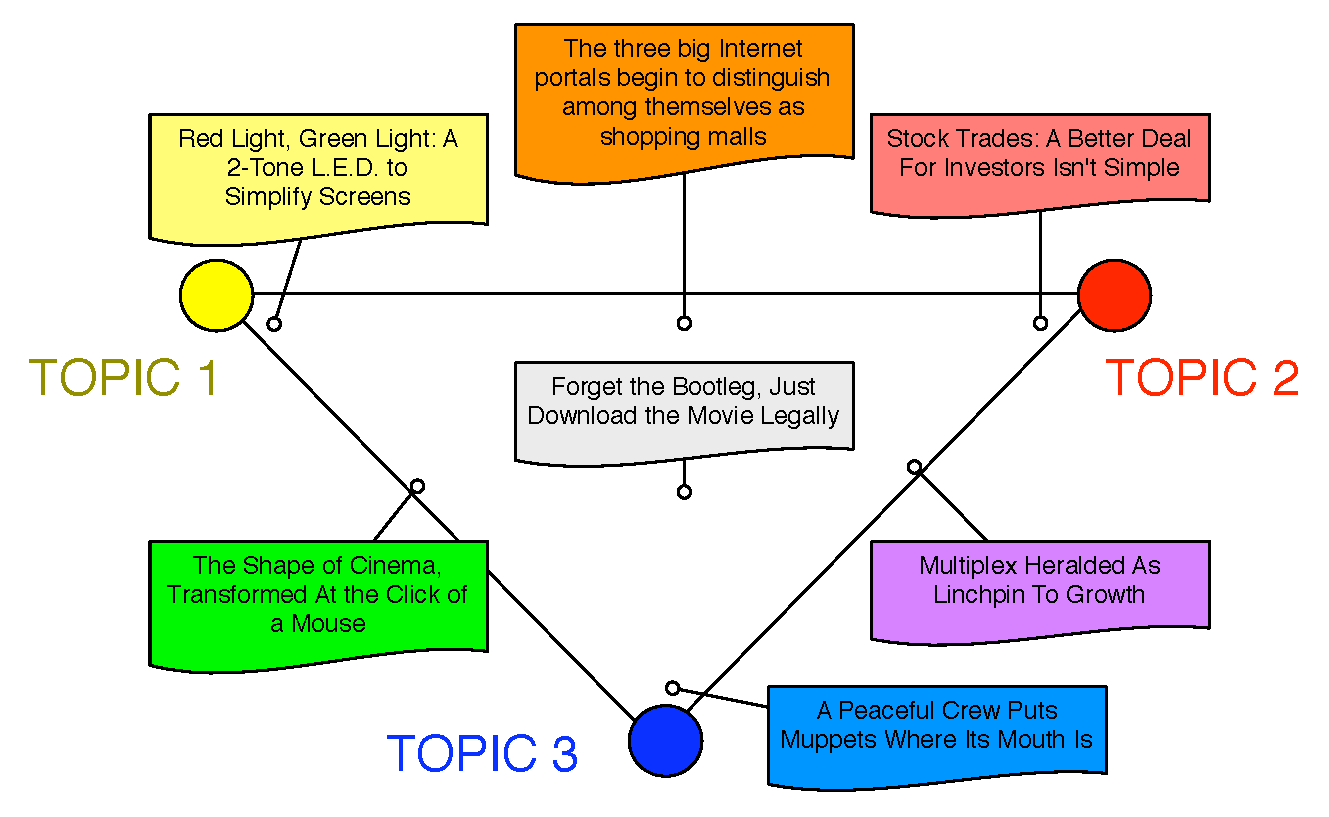
\includegraphics[width=0.7\linewidth]{topic_models/nyt_documents}
        \end{block}

\end{frame}

\begin{frame}

\frametitle{Dirichlet Distribution}

\begin{center}
\begin{equation}
  p(\theta | \vec{\alpha}) = \frac{ \Gamma \left( \sum_k \alpha_k \right)}{\prod_k \Gamma(\alpha_k)} \prod_k \theta_k^{\alpha_k - 1}
\end{equation}
\bigskip

\only<2>{
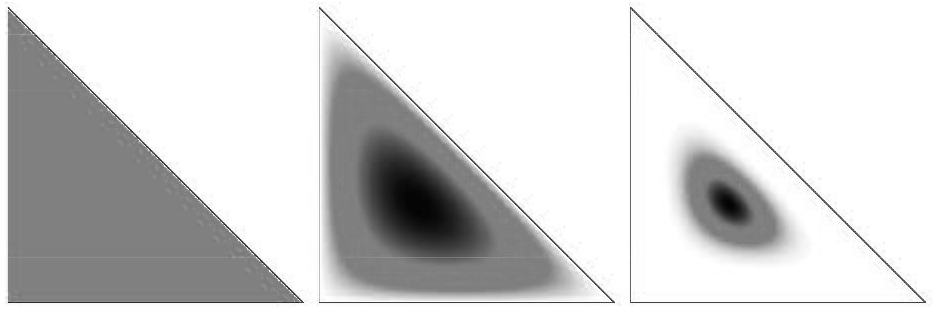
\includegraphics[width=0.6\linewidth]{topic_models/dirichlet_1} \\
\begin{tabular}{ccc}
$\vec \alpha = \left(1, 1, 1 \right)$ &
$\vec \alpha = \left(2, 2, 2 \right)$ & 
$\vec \alpha = \left(10, 10, 10 \right)$  \\
\end{tabular} }

\only<3>{
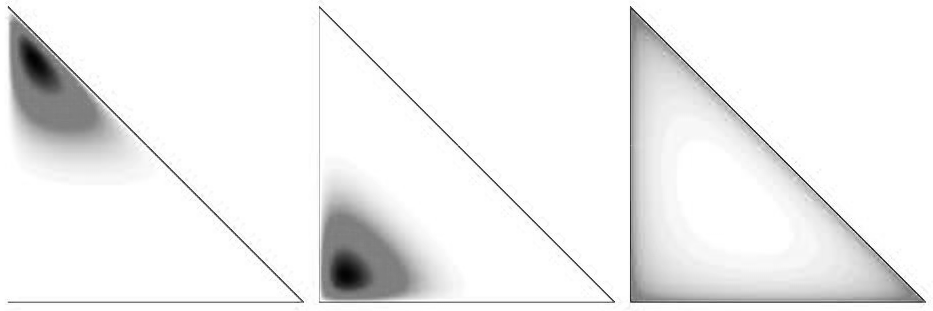
\includegraphics[width=0.6\linewidth]{topic_models/dirichlet_2} \\
\begin{tabular}{ccc}
$\vec \alpha = \left(2, 10, 2 \right)$ & 
$\vec \alpha = \left(2, 2, 10 \right)$ & 
$\vec \alpha = \left(\frac{4}{5}, \frac{4}{5}, \frac{4}{5} \right)$  \\
\end{tabular} }

\only<4>{Intuition: Documents only talk about a handful of topics.}

\end{center}

\end{frame}


\fi
\ifconjugacy

\begin{frame}
\frametitle{Dirichlet Distribution}
\begin{itemize}
  \item If ${\bm \phi} \sim \Dir(\alpha)$, ${\bm w} \sim \Mult(\phi)$, and $n_k = |\{ w_i : w_i = k\}|$ then
  \begin{align}
  	p(\phi | \alpha, {\bm w}) & \propto p({\bm w} | \phi) p(\phi | \alpha) \\
	                       & \propto  \prod_{k} \phi^{n_k} \pause  \prod_k { \phi^{\alpha_k - 1}} \\
	                       & \propto \prod_k \phi^{\alpha_k + n_k - 1}
  \end{align}
  \item Conjugacy: this {\bf posterior} has the same form as the {\bf prior}
\end{itemize}
\end{frame}

\fi

\ifhighlevel

\else

\begin{frame}{Generative Model}
  \centering
	\only<1> {   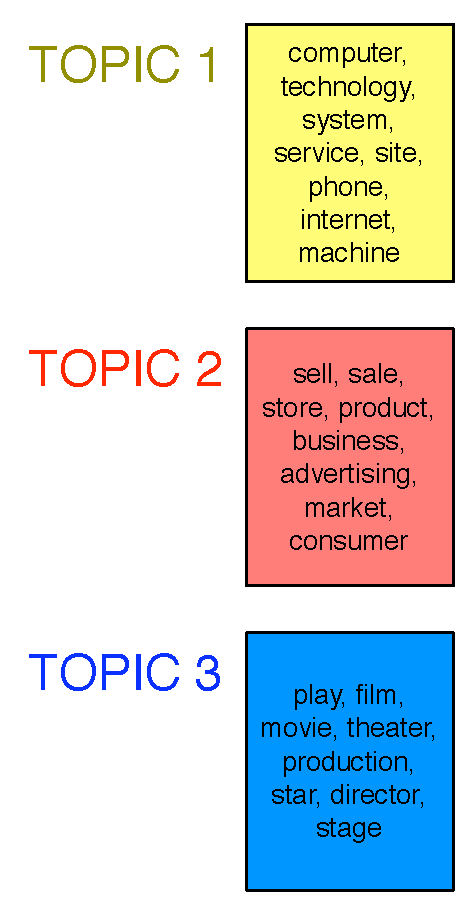
\includegraphics[width=.3\linewidth]{topic_models/nyt_topics}  }
	\only<2> {   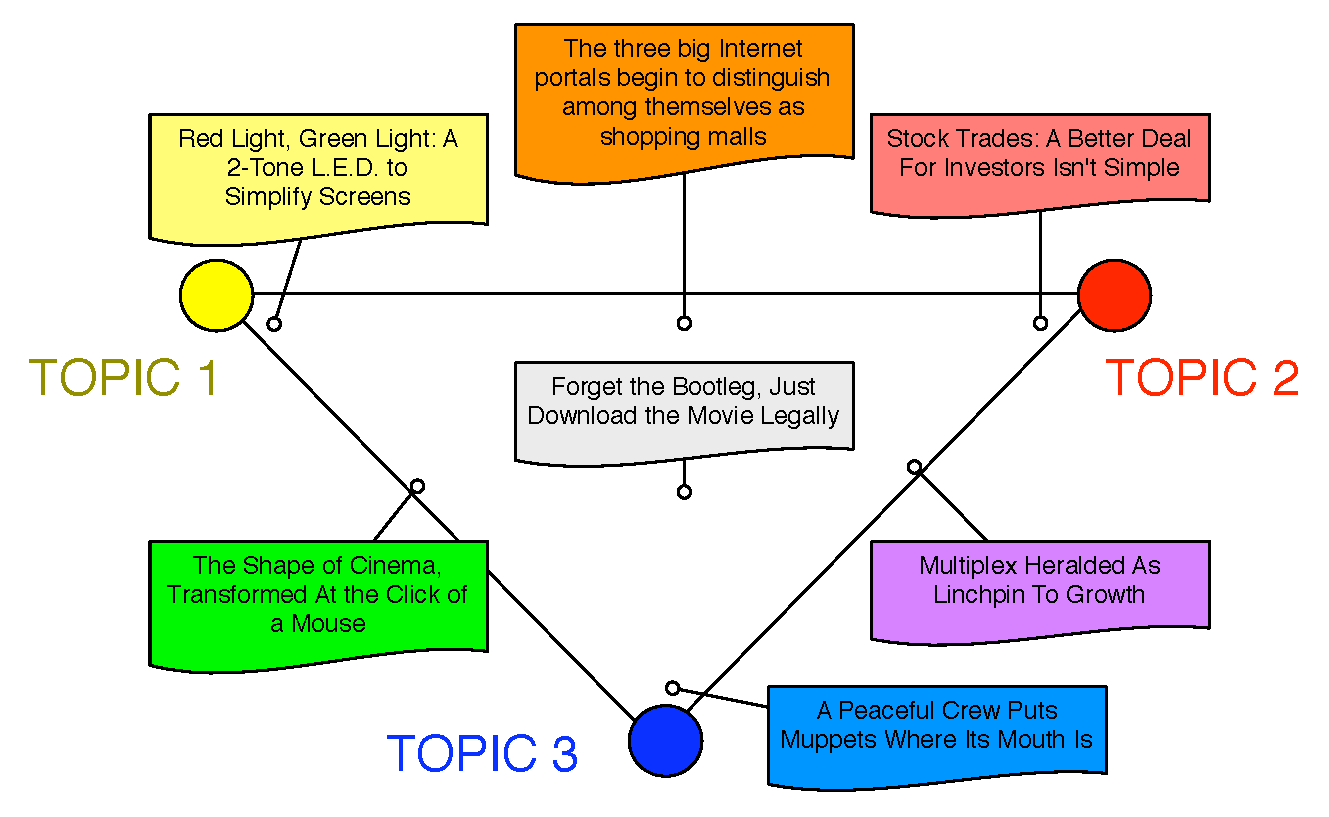
\includegraphics[width=.9\linewidth]{topic_models/nyt_documents}  }
	\only<3> {   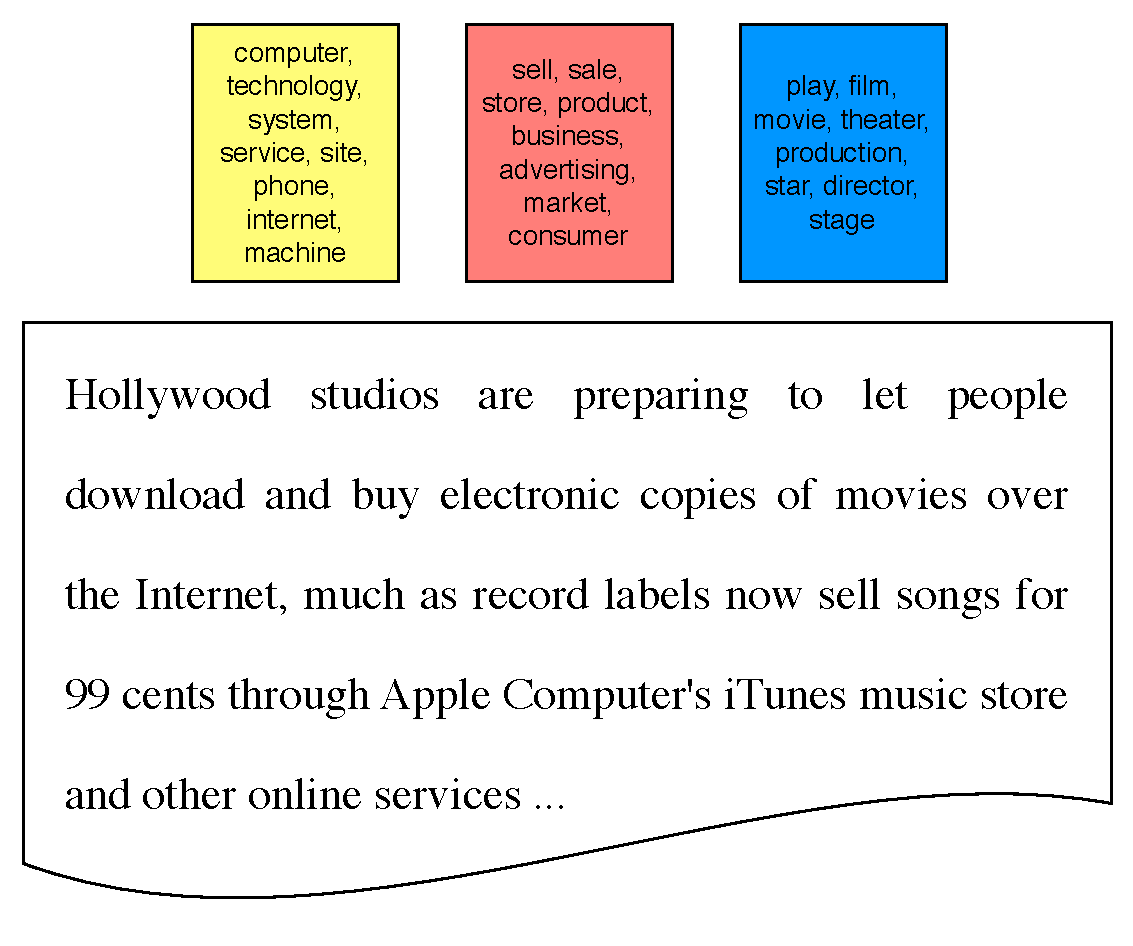
\includegraphics[width=.8\linewidth]{topic_models/inference_0}  }
	\only<4> {   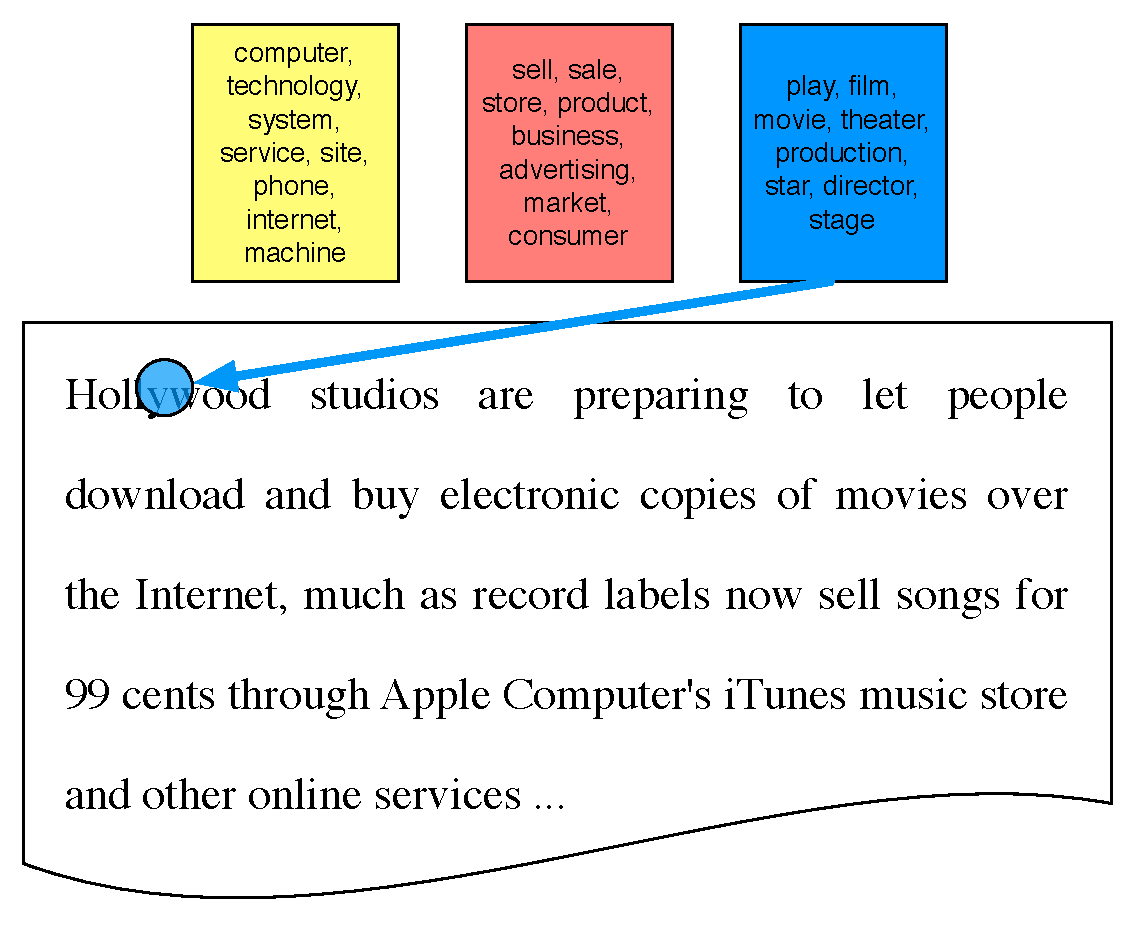
\includegraphics[width=.8\linewidth]{topic_models/inference_1}  }
	\only<5> {   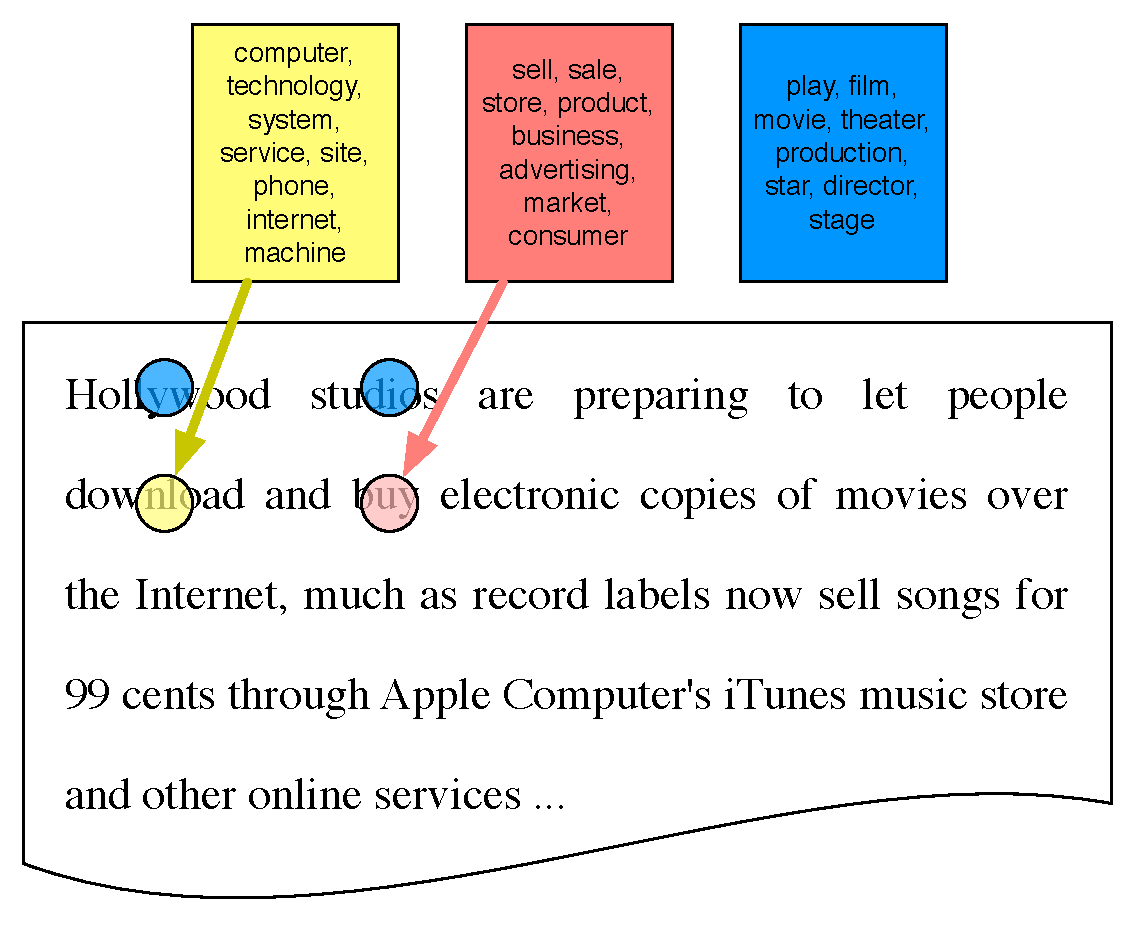
\includegraphics[width=.8\linewidth]{topic_models/inference_2}  }
	\only<6> {   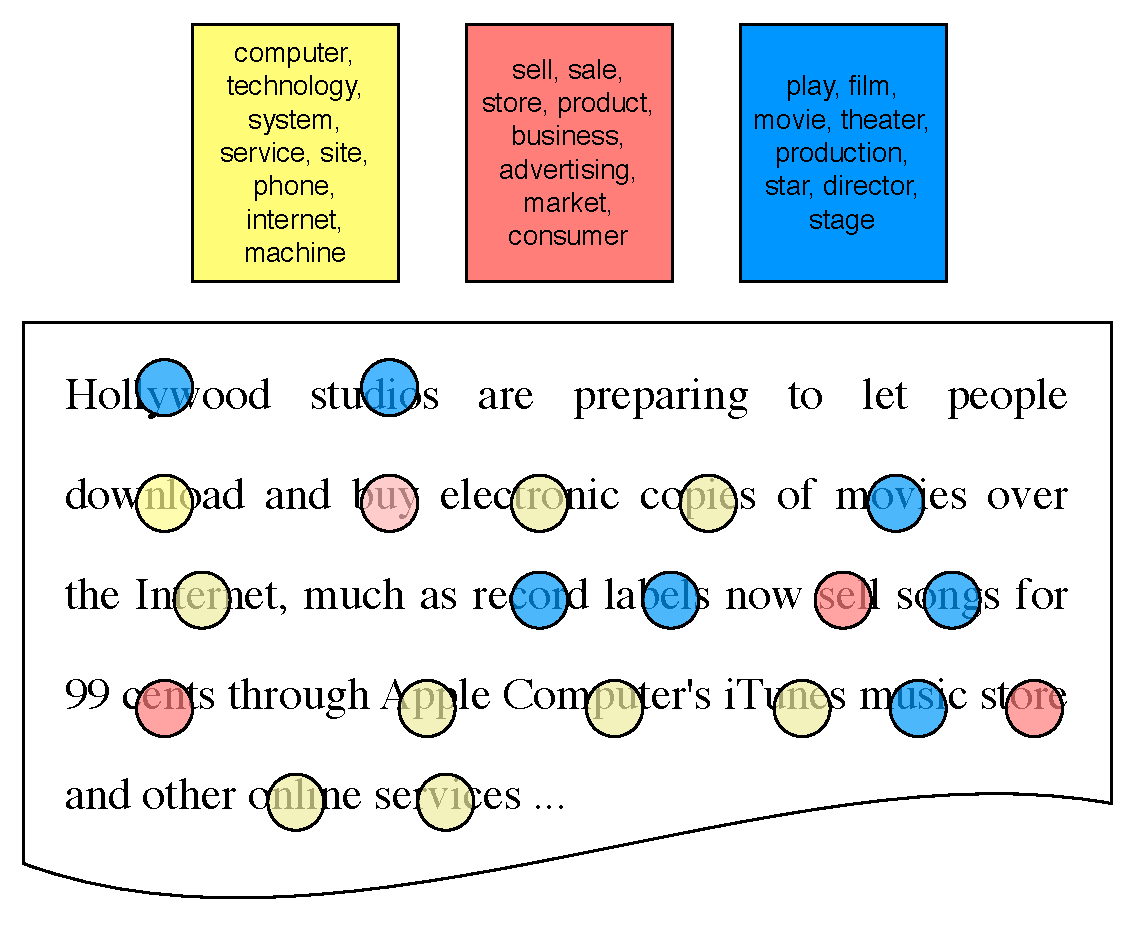
\includegraphics[width=.8\linewidth]{topic_models/inference_3}  }


\end{frame}

\frame
{
  \frametitle{Generative Model Approach}

\begin{center}
\only<1>{ 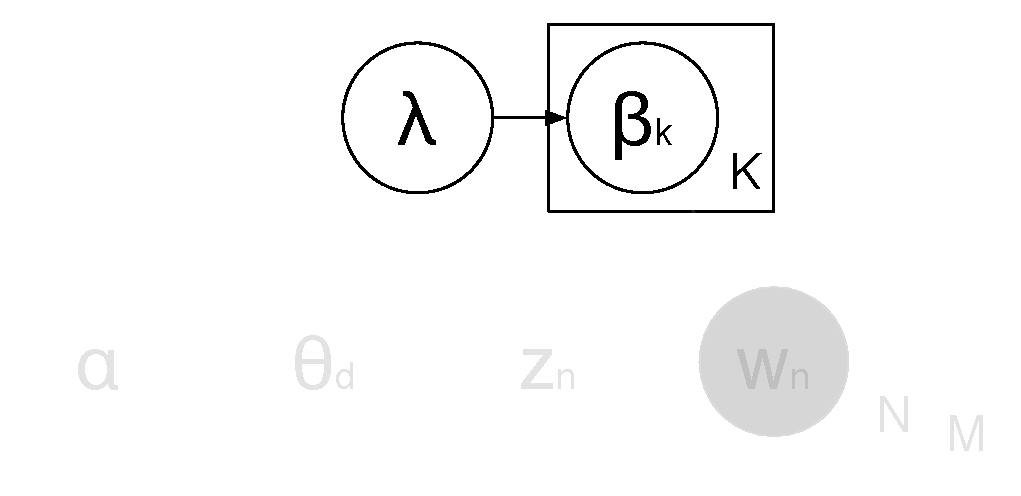
\includegraphics[scale=0.4]{topic_models/lda1.pdf} }
\only<2>{ 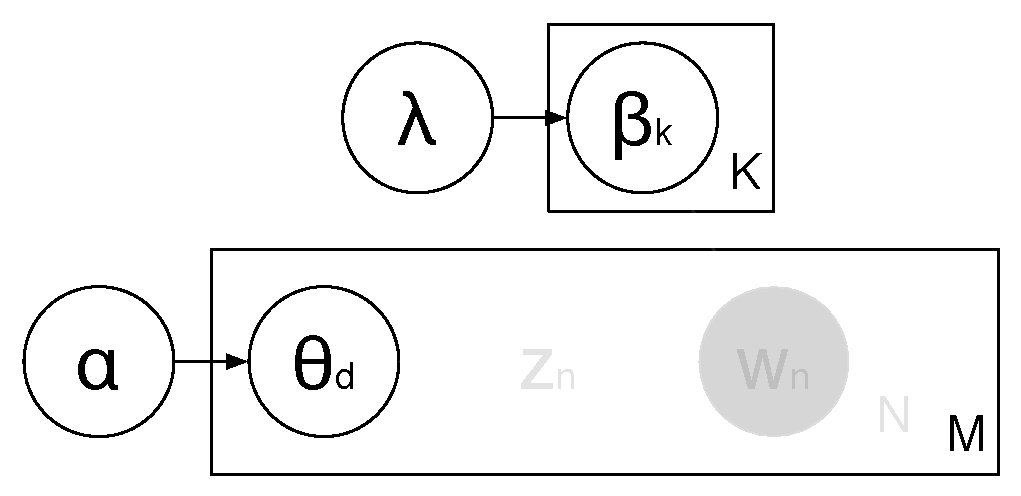
\includegraphics[scale=0.4]{topic_models/lda2.pdf} }
\only<3>{ 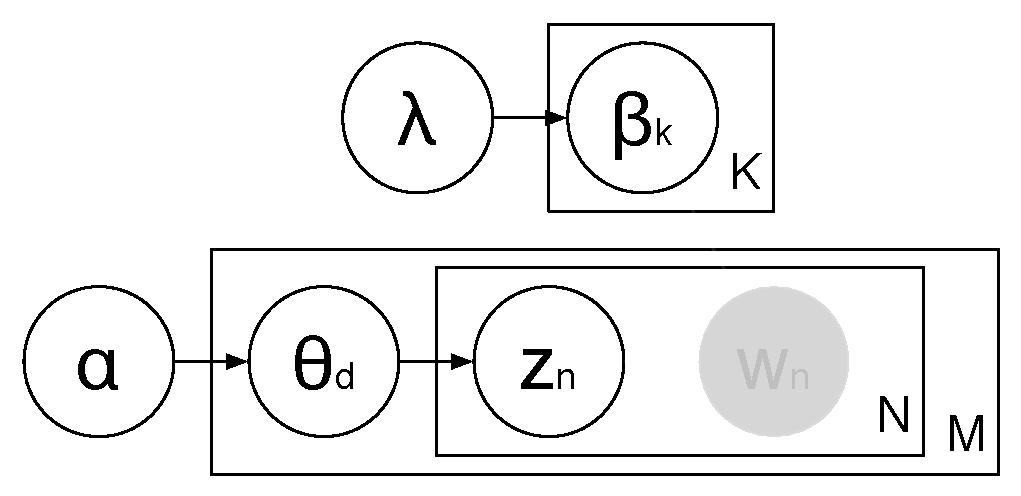
\includegraphics[scale=0.4]{topic_models/lda3.pdf} }
\only<4->{ 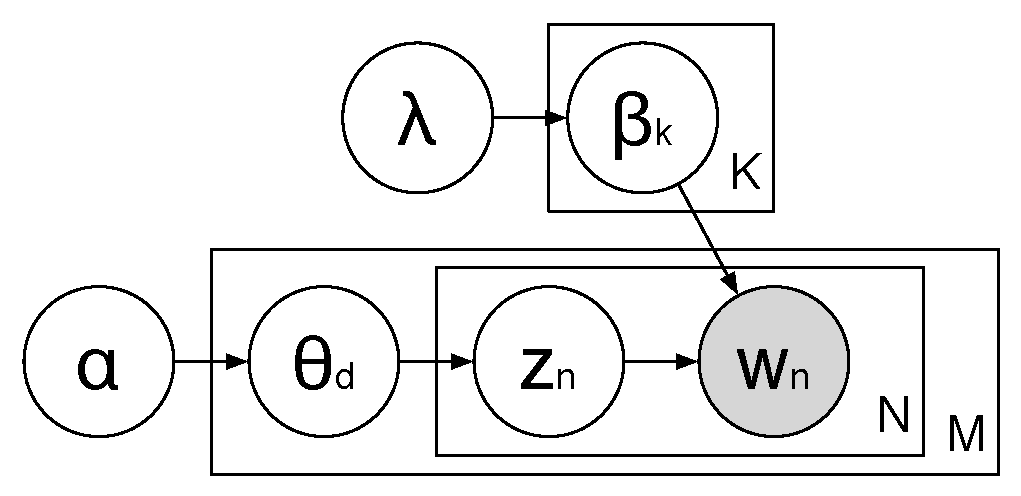
\includegraphics[scale=0.4]{topic_models/lda4.pdf} }
\end{center}

\begin{itemize}
\item<1-> For each topic $k \in \{1, \dots, K\}$, draw a multinomial distribution $\beta_k$ from a Dirichlet distribution with parameter $\lambda$
\item<2-> For each document $d \in \{1, \dots, M\}$, draw a multinomial distribution $\theta_d$ from a Dirichlet distribution with parameter $\alpha$
\item<3-> For each word position $n \in \{1, \dots, N\}$, select a hidden topic $z_n$ from the multinomial distribution parameterized by $\theta$.
\item<4-> Choose the observed word $w_n$ from the distribution $\beta_{z_n}$.
\end{itemize}

\only<5->{We use statistical inference to uncover the most likely unobserved variables given observed data.}
}

\fi

\begin{frame}
\frametitle{Topic Models: What's Important}
\begin{itemize}
\item Topic models \only<2>{(latent variables)}
\begin{itemize}
\ifhighlevel
	\item Topics to words
	\item Documents to topics
\else
	\item Topics to words---multinomial distribution
	\item Documents to topics---multinomial distribution
\fi
\end{itemize}
\item Focus in this talk: statistical methods
  \begin{itemize}
    \item Model: story of how your data came to be
    \item Latent variables: missing pieces of your story
    \item Statistical inference: filling in those missing pieces
  \end{itemize}
\item We use latent Dirichlet allocation (LDA)~\cite{blei-03}, a fully Bayesian
  version of pLSI~\cite{hofmann-99}, probabilistic version of
  LSA~\cite{landauer-97}
\end{itemize}

\end{frame}

\ifevaluation


\frame{
\frametitle{Evaluation}
\begin{center}
%\only<1>{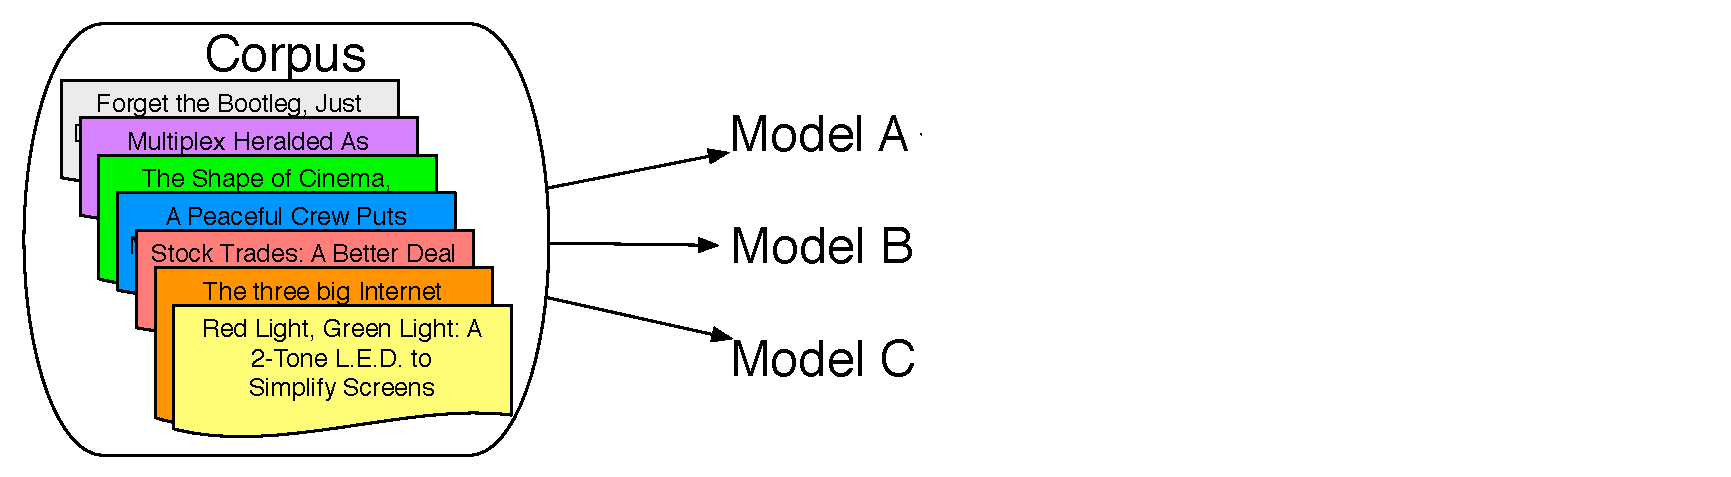
\includegraphics[width=0.9\linewidth]{reading_tea_leaves/figures/heldout_1} }
\only<1>{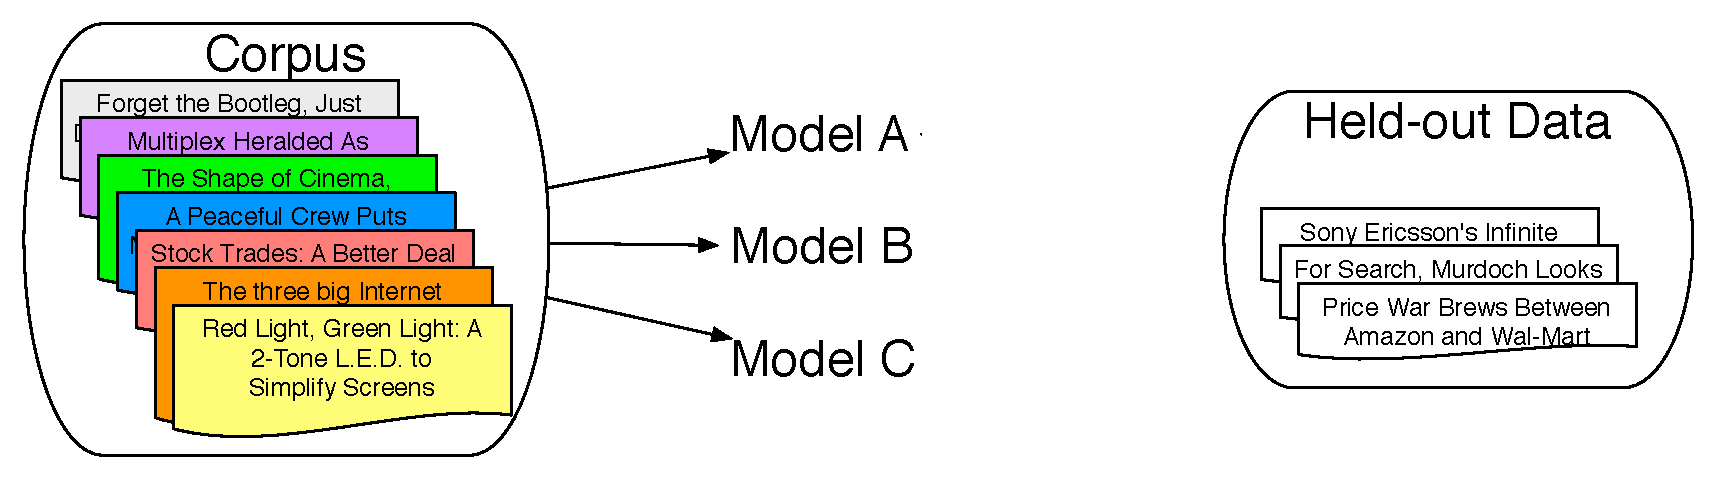
\includegraphics[width=\linewidth]{reading_tea_leaves/figures/heldout_2} }
%\only<3>{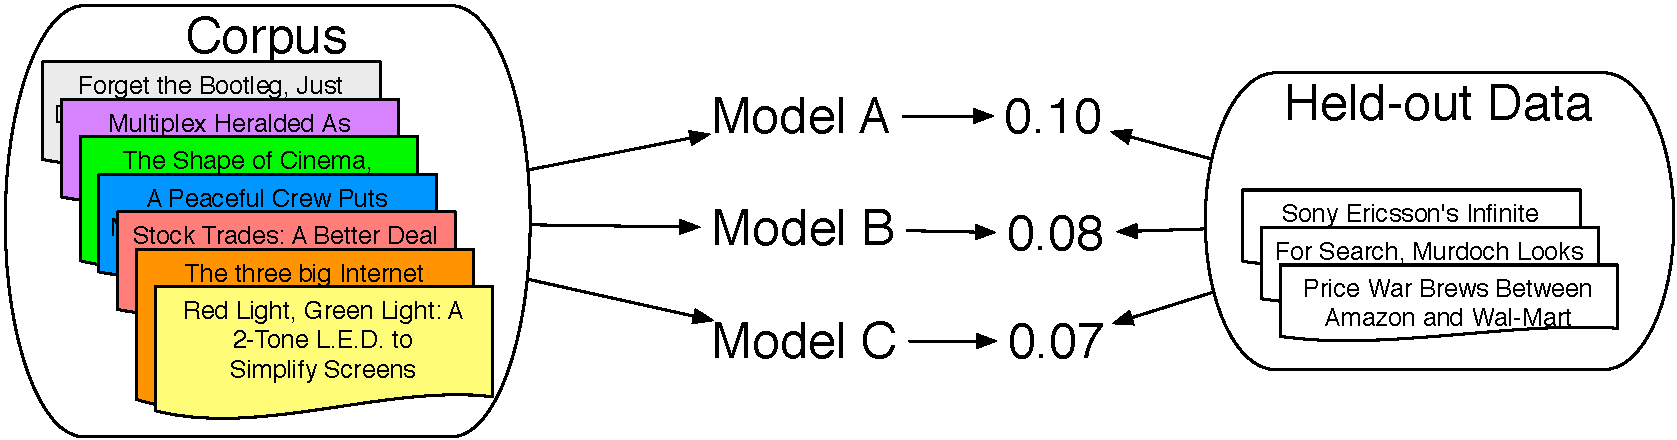
\includegraphics[width=\linewidth]{reading_tea_leaves/figures/heldout_3} }
\only<2>{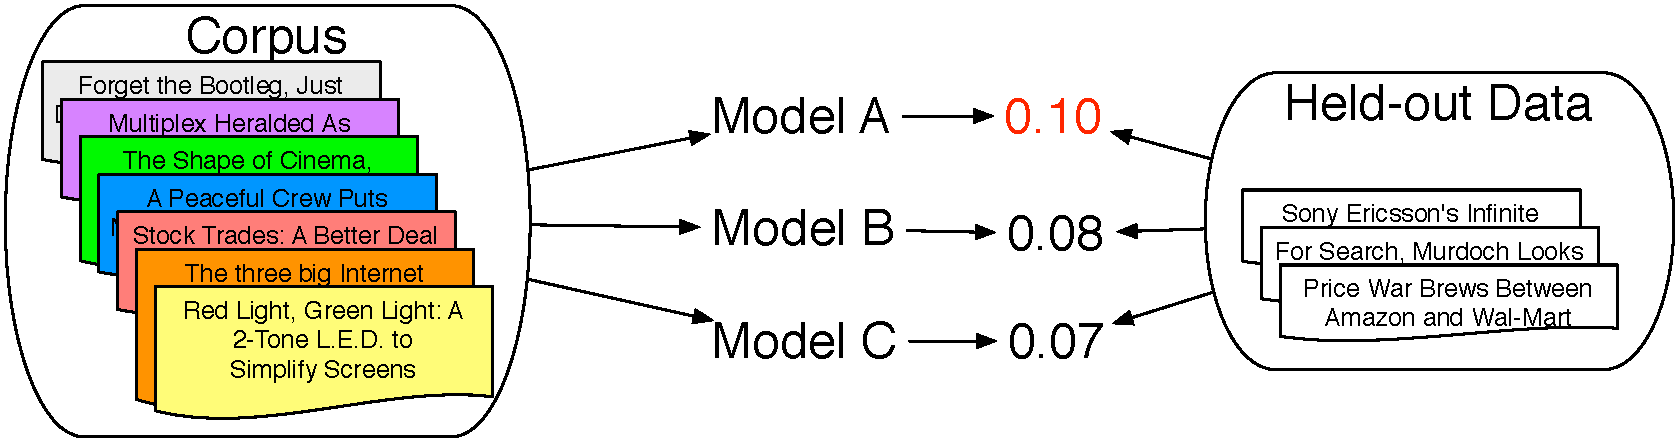
\includegraphics[width=\linewidth]{reading_tea_leaves/figures/heldout_4}  \\
	\large Measures predictive power, not what the topics are}
\end{center}

\begin{center}
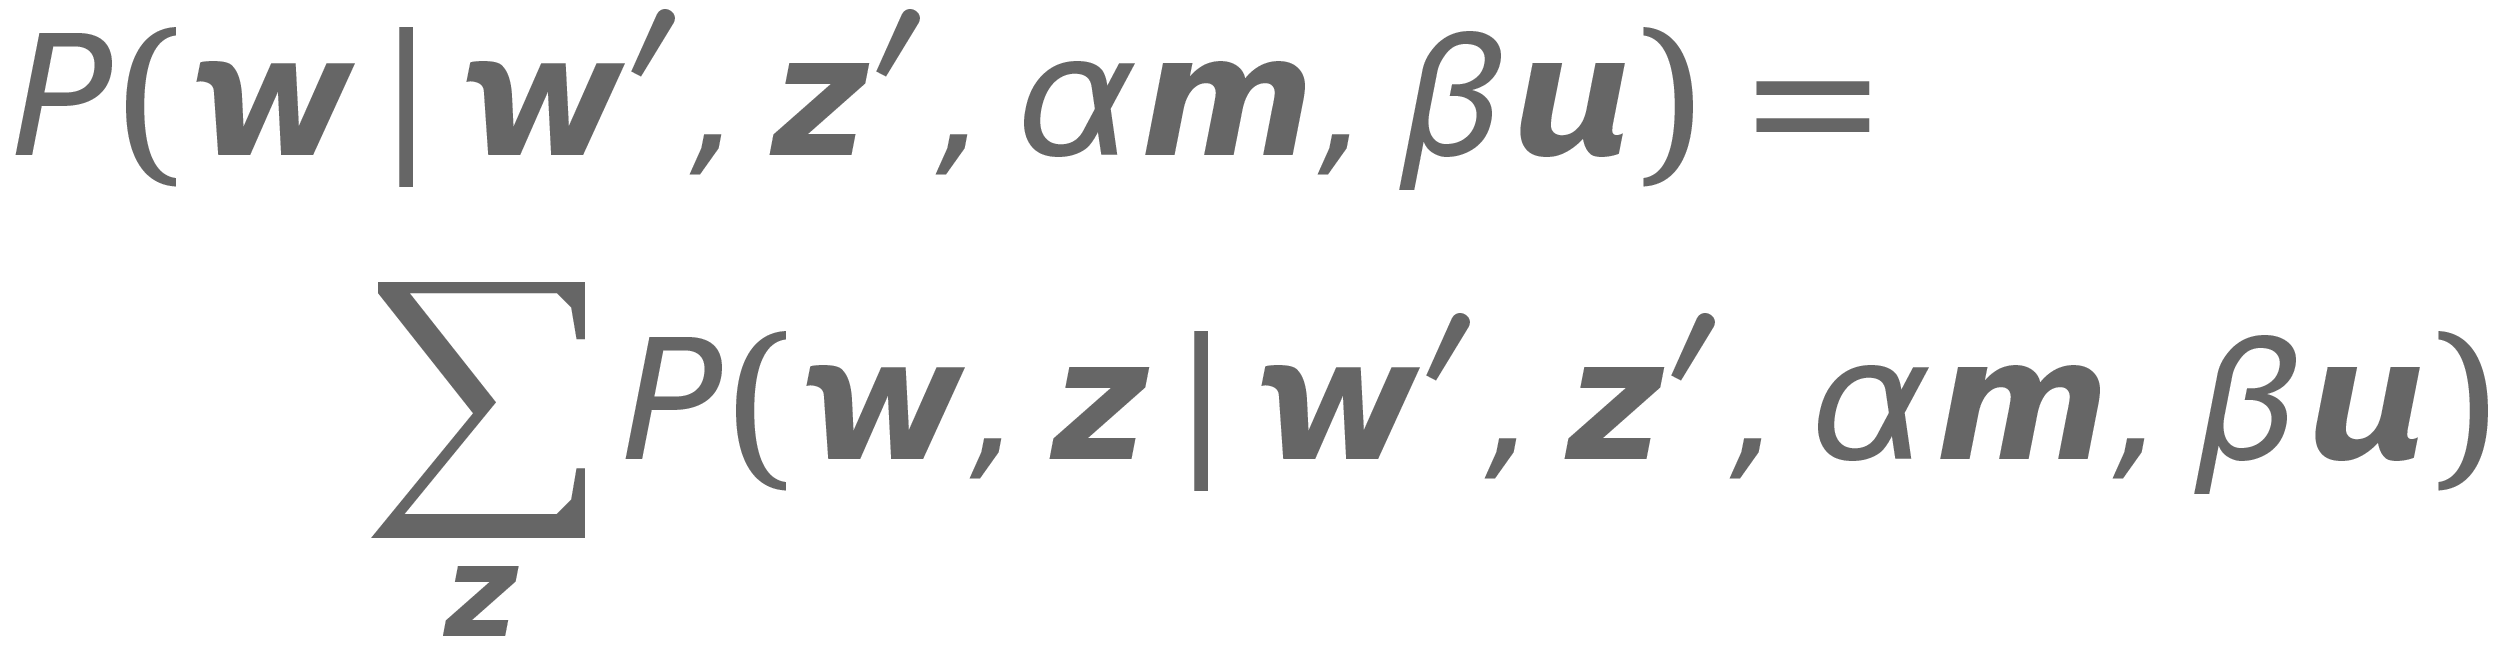
\includegraphics[width=0.5\linewidth]{topic_models/equations/evaluation} \\
How you compute it is important too~\cite{wallach-09b}
\end{center}

}

\frame{
  \frametitle{Word Intrusion}

  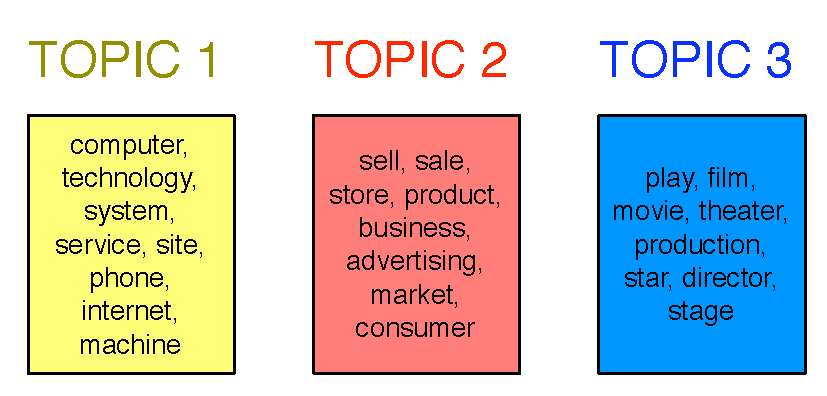
\includegraphics[width=\linewidth]{reading_tea_leaves/figures/nyt_topics_wide}
}


\frame{
  \frametitle{Word Intrusion}

  \begin{enumerate}
    \item Take the highest probability words from a topic

      \begin{block}{Original Topic}
        dog, cat, horse, pig, cow
      \end{block}
\pause
    \item Take a high-probability word from another topic and add it
      \begin{block}{Topic with Intruder}
        dog, cat, \alert<2->{apple}, horse, pig, cow
      \end{block}
\pause
     \item We ask users to find the word that doesn't belong
  \end{enumerate}
\begin{block}{Hypothesis}
If the topics are interpretable, users will consistently choose true intruder
\end{block}
}

\frame{
\frametitle{Word Intrusion}
\begin{center}
\only<1>{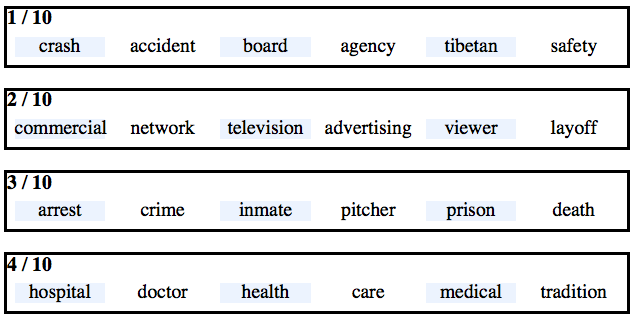
\includegraphics[width=\linewidth]{reading_tea_leaves/tasks/word1}  }
\only<2>{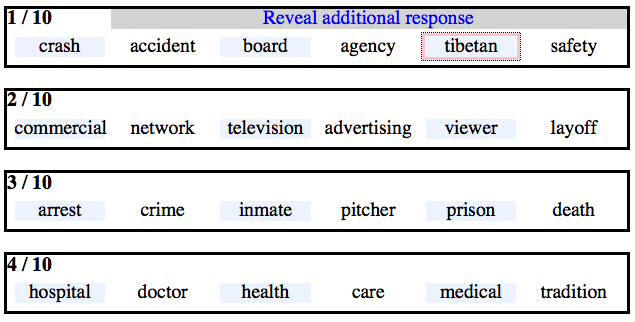
\includegraphics[width=\linewidth]{reading_tea_leaves/tasks/word2}  }
\pause
  \begin{itemize}
    \item Order of words was shuffled
    \item Which intruder was selected varied
    \item Model precision: percentage of users who clicked on intruder
  \end{itemize}

\end{center}
}

\frame{
\frametitle{Word Intrusion: Which Topics are Interpretable?}
  \begin{block}{New York Times, 50 LDA Topics}
    \begin{center}
      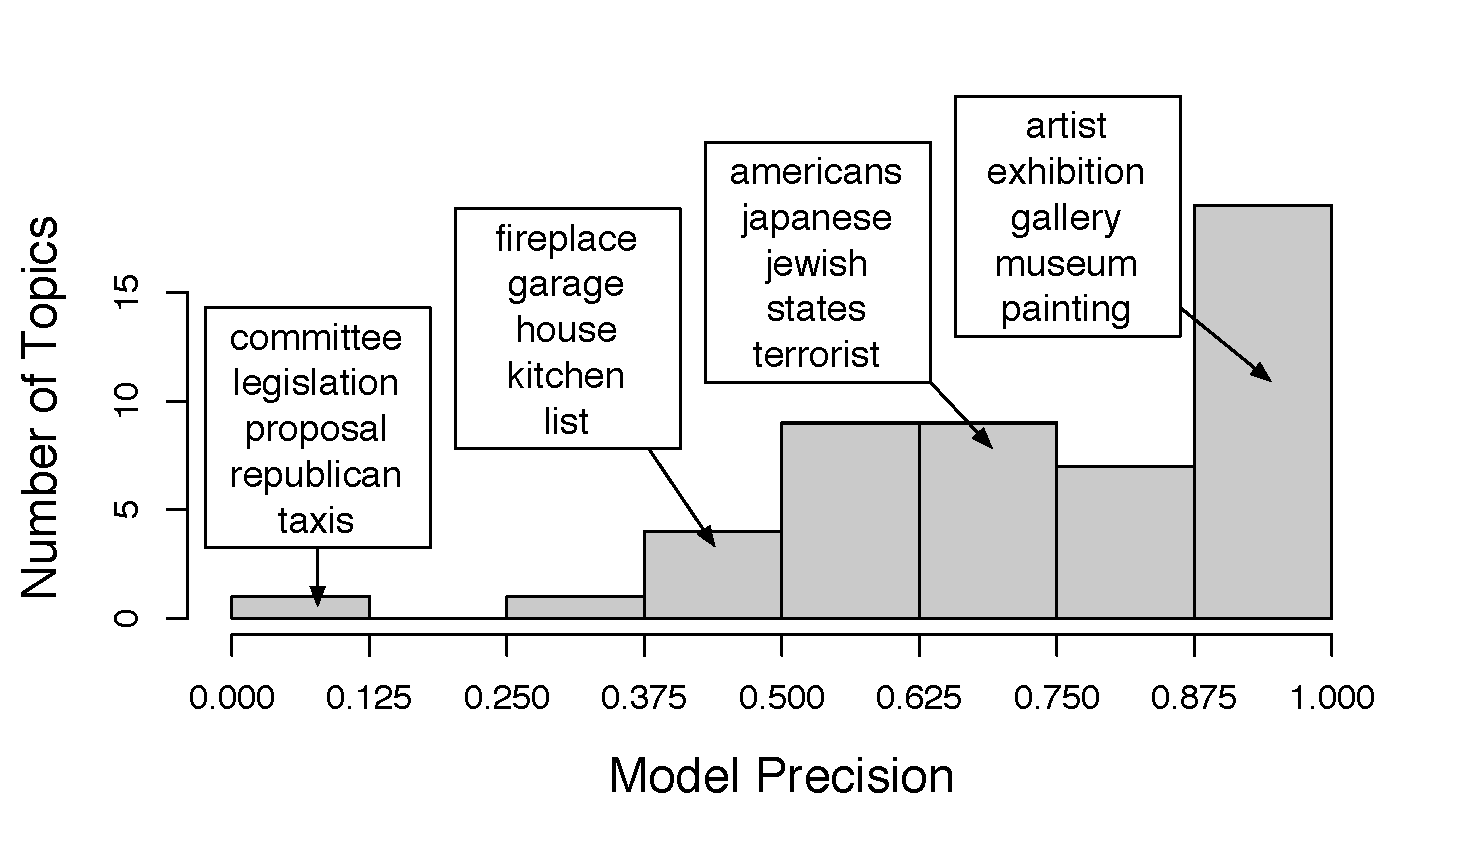
\includegraphics[width=0.8\linewidth]{reading_tea_leaves/figures/topic_precision}
    \end{center}
  \end{block}
  \begin{center}
    Model Precision: percentage of correct intruders found
  \end{center}
}



\frame{

\frametitle{Interpretability and Likelihood}
\begin{center}
\only<1>{Model Precision on New York Times}
\only<2>{Topic Log Odds on Wikipedia}
\end{center}

\begin{columns}
\column{.85\linewidth}
\begin{flushright}
  \only<1>{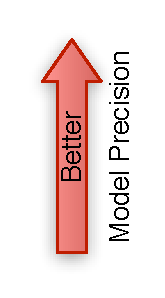
\includegraphics[scale=\graphscale]{reading_tea_leaves/tasks/mp}}
  \only<2>{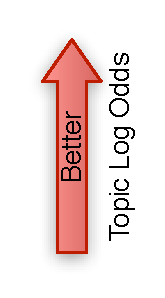
\includegraphics[scale=\graphscale]{reading_tea_leaves/tasks/tlo}}
  \only<1>{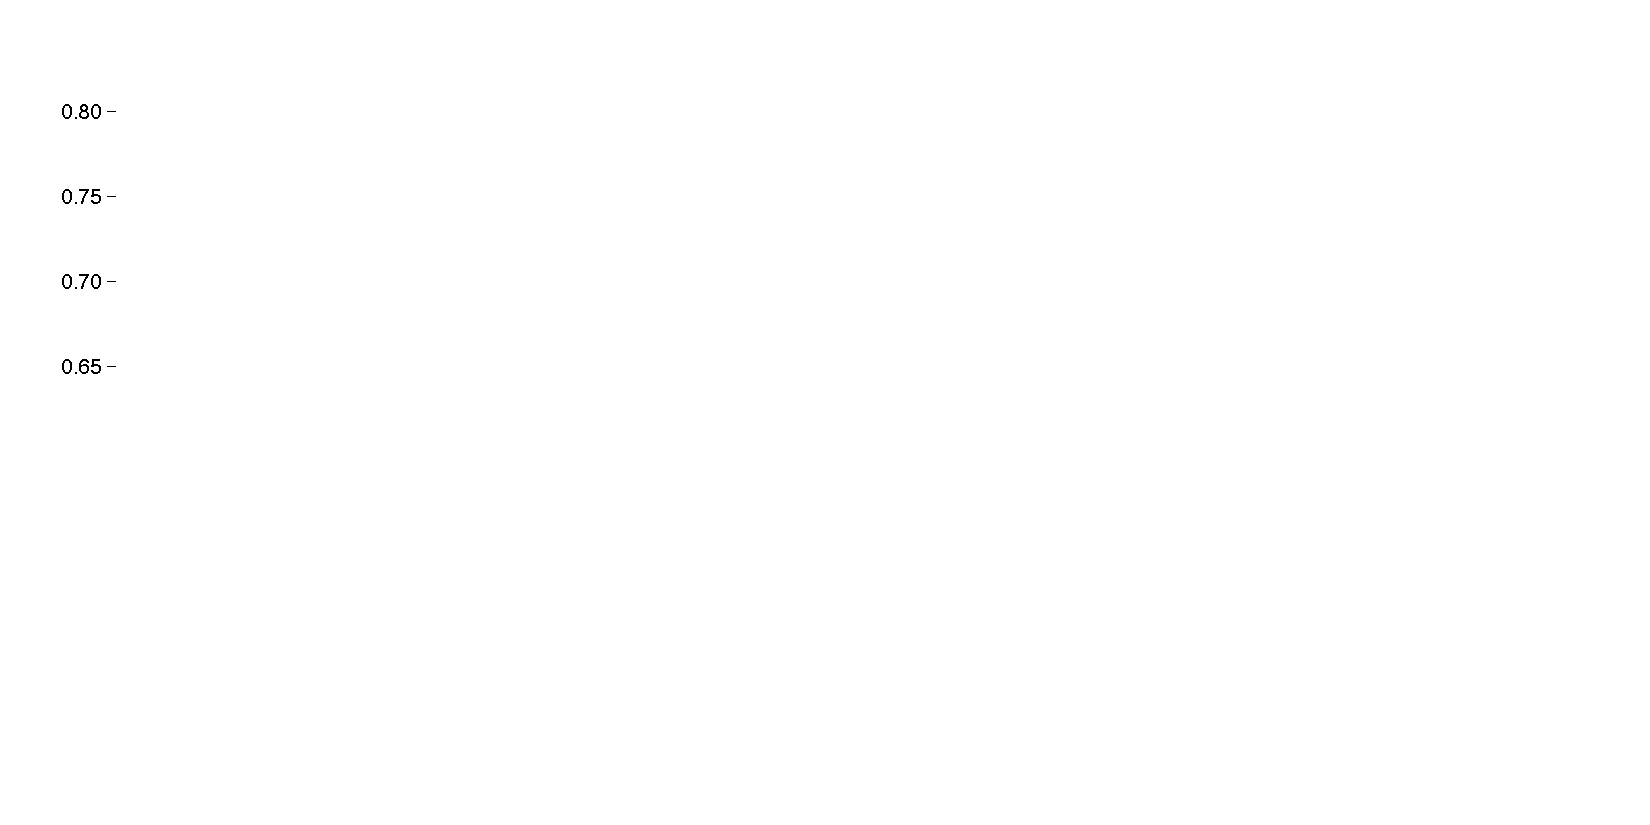
\includegraphics[scale=\graphscale]{reading_tea_leaves/tasks/mp_y}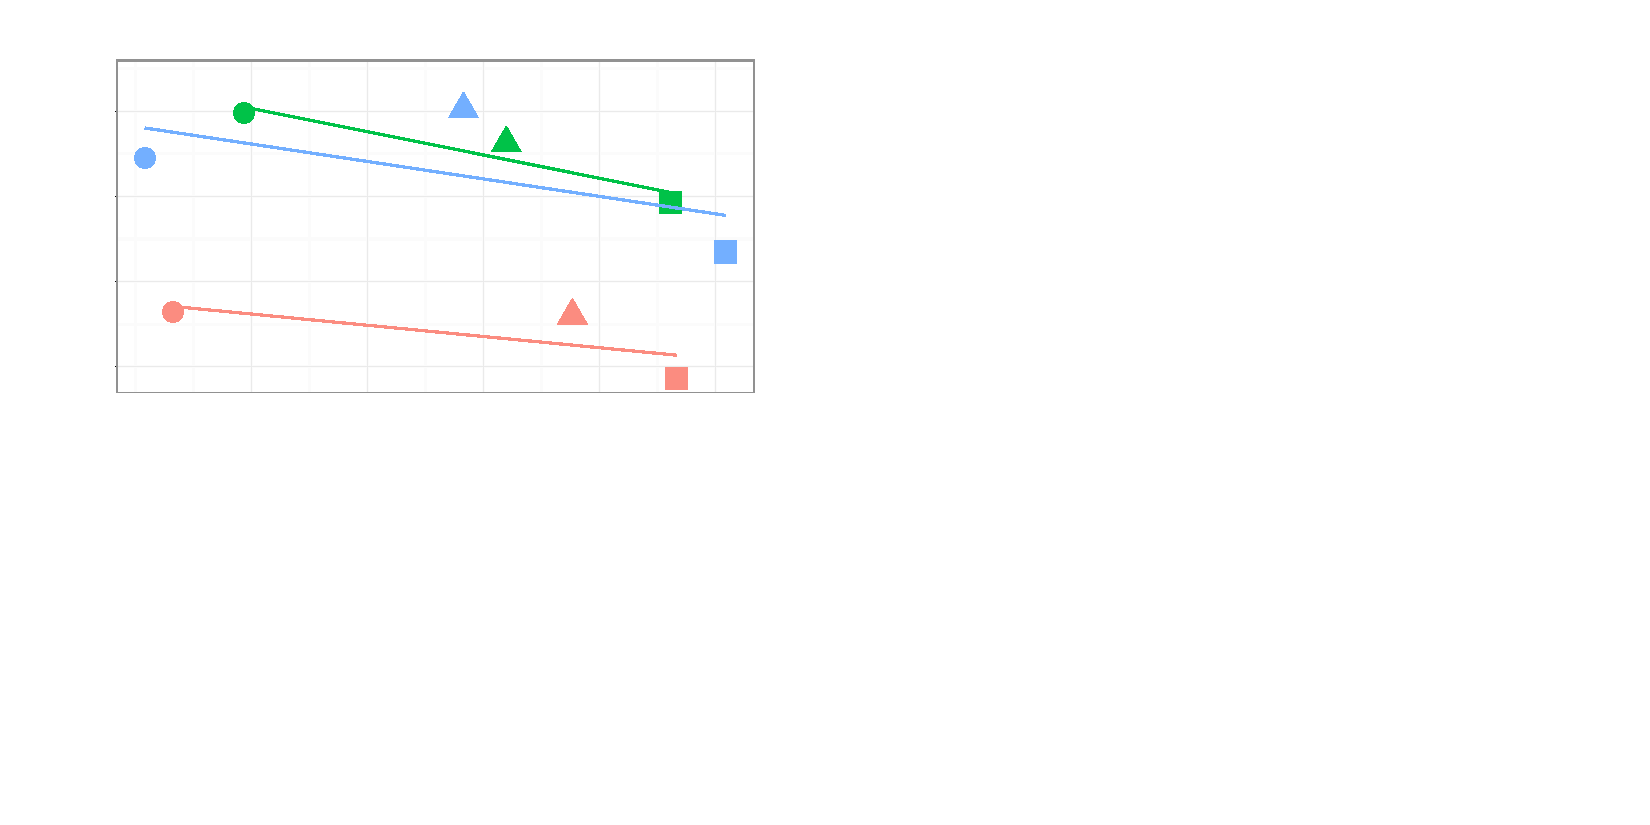
\includegraphics[scale=\graphscale]{reading_tea_leaves/tasks/nyt_mp}}
  \only<2>{
\includegraphics[scale=\graphscale]{reading_tea_leaves/tasks/tlo_y}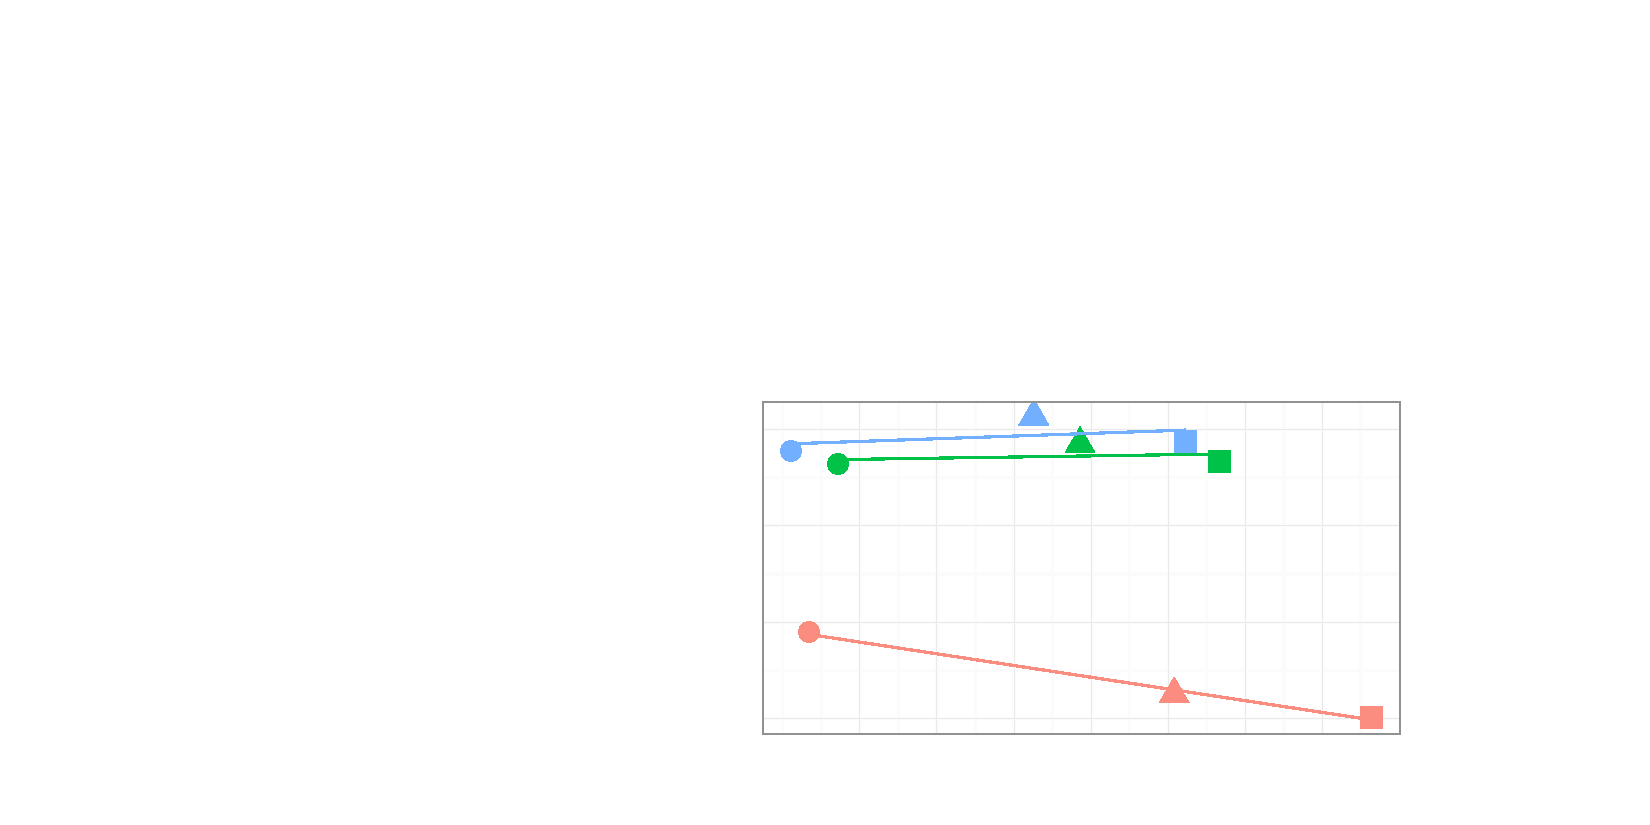
\includegraphics[scale=\graphscale]{reading_tea_leaves/tasks/wiki_tlo}} \\
  \only<1>{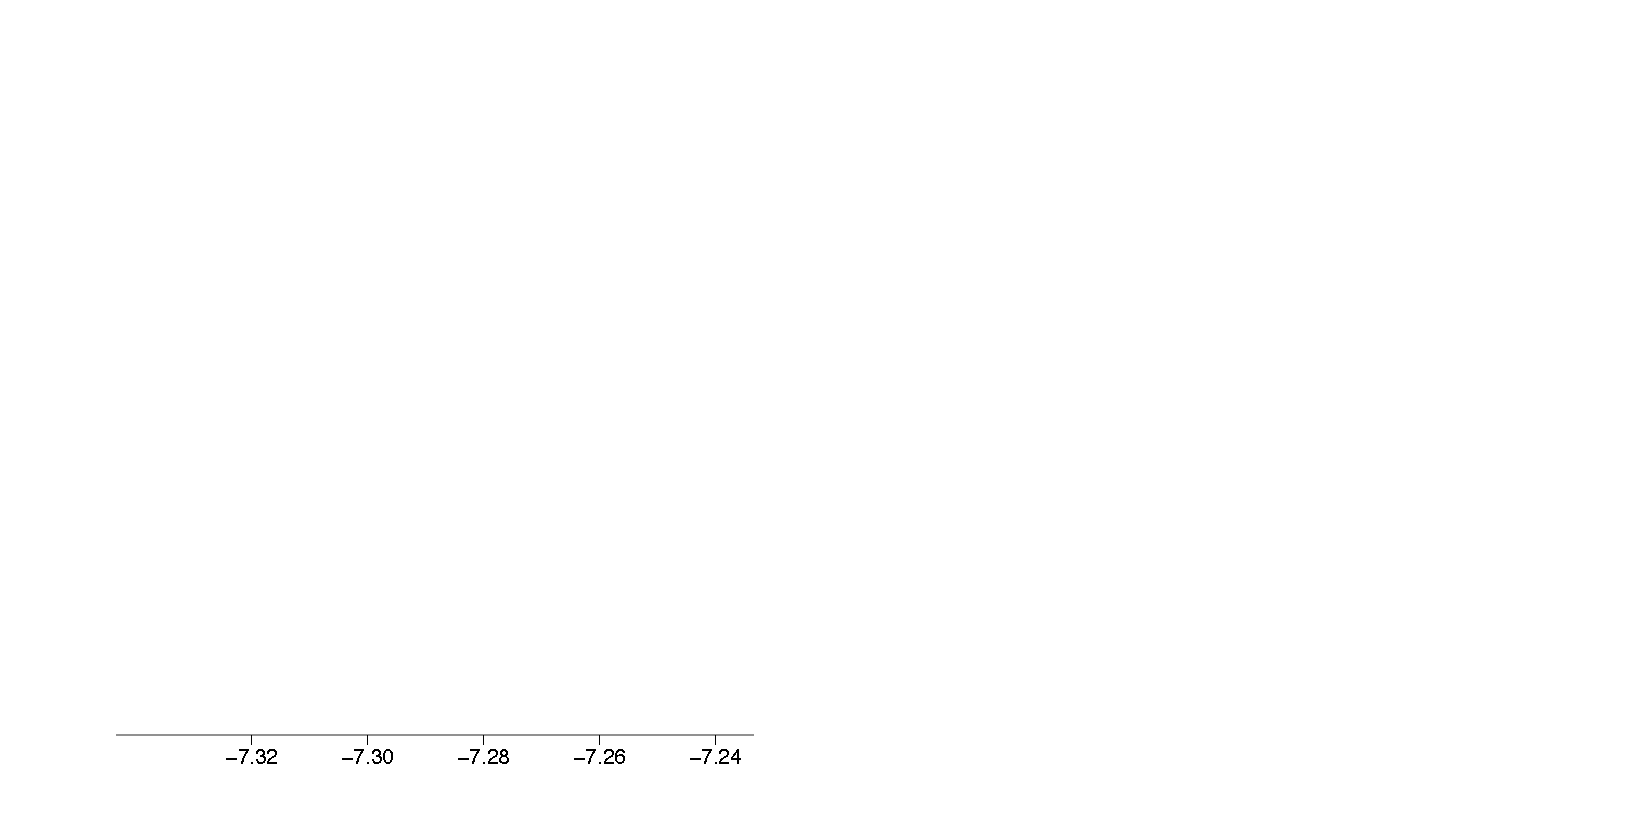
\includegraphics[scale=\graphscale]{reading_tea_leaves/tasks/nyt_x}}
  \only<2>{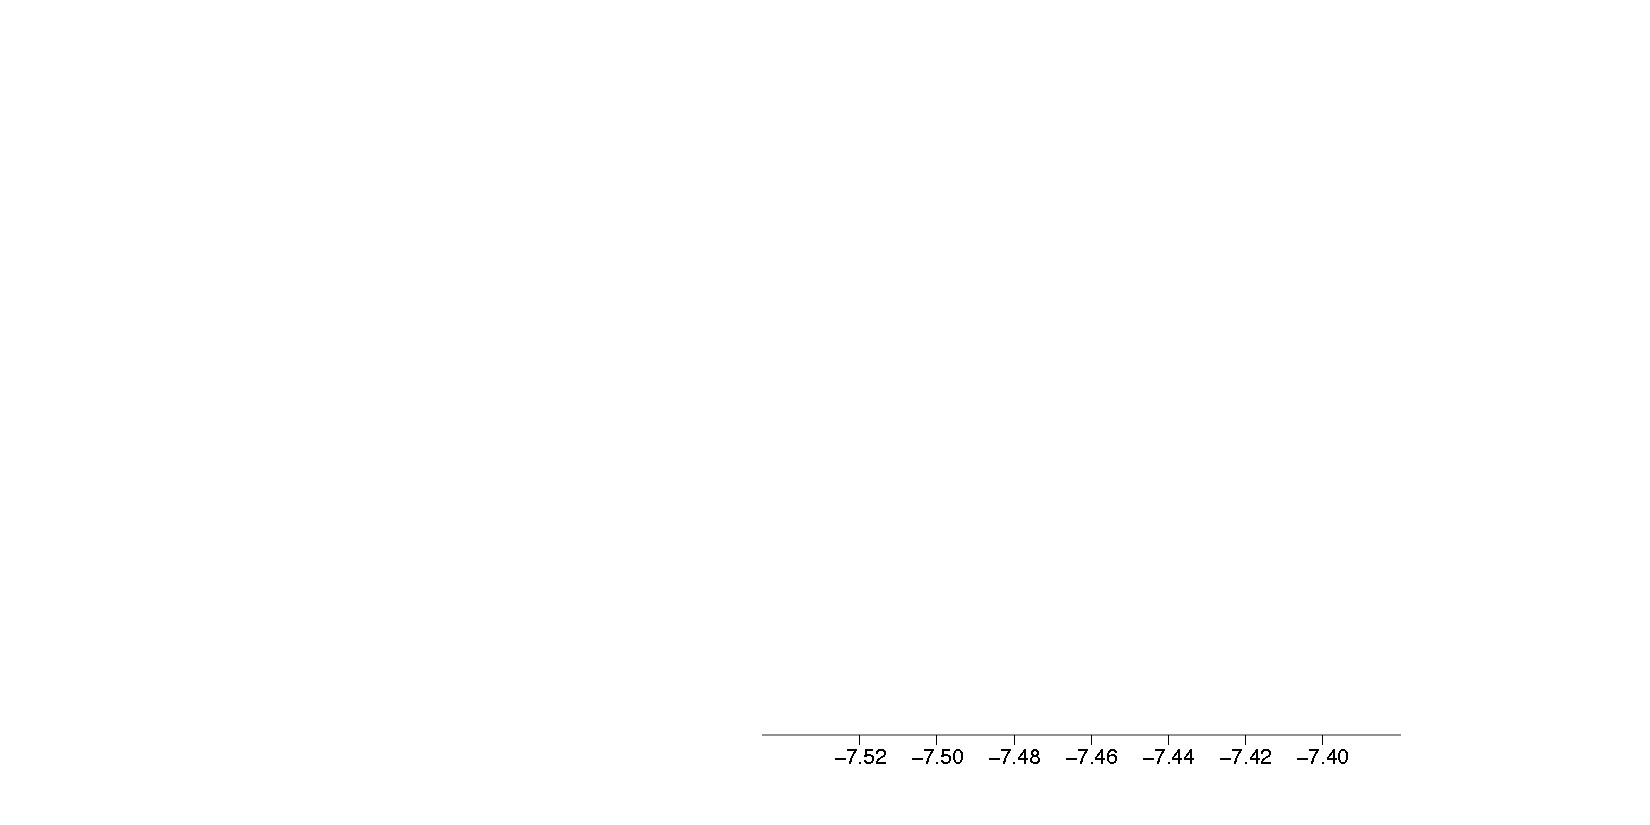
\includegraphics[scale=\graphscale]{reading_tea_leaves/tasks/wiki_x}}
\end{flushright}
\column{.15\linewidth}
  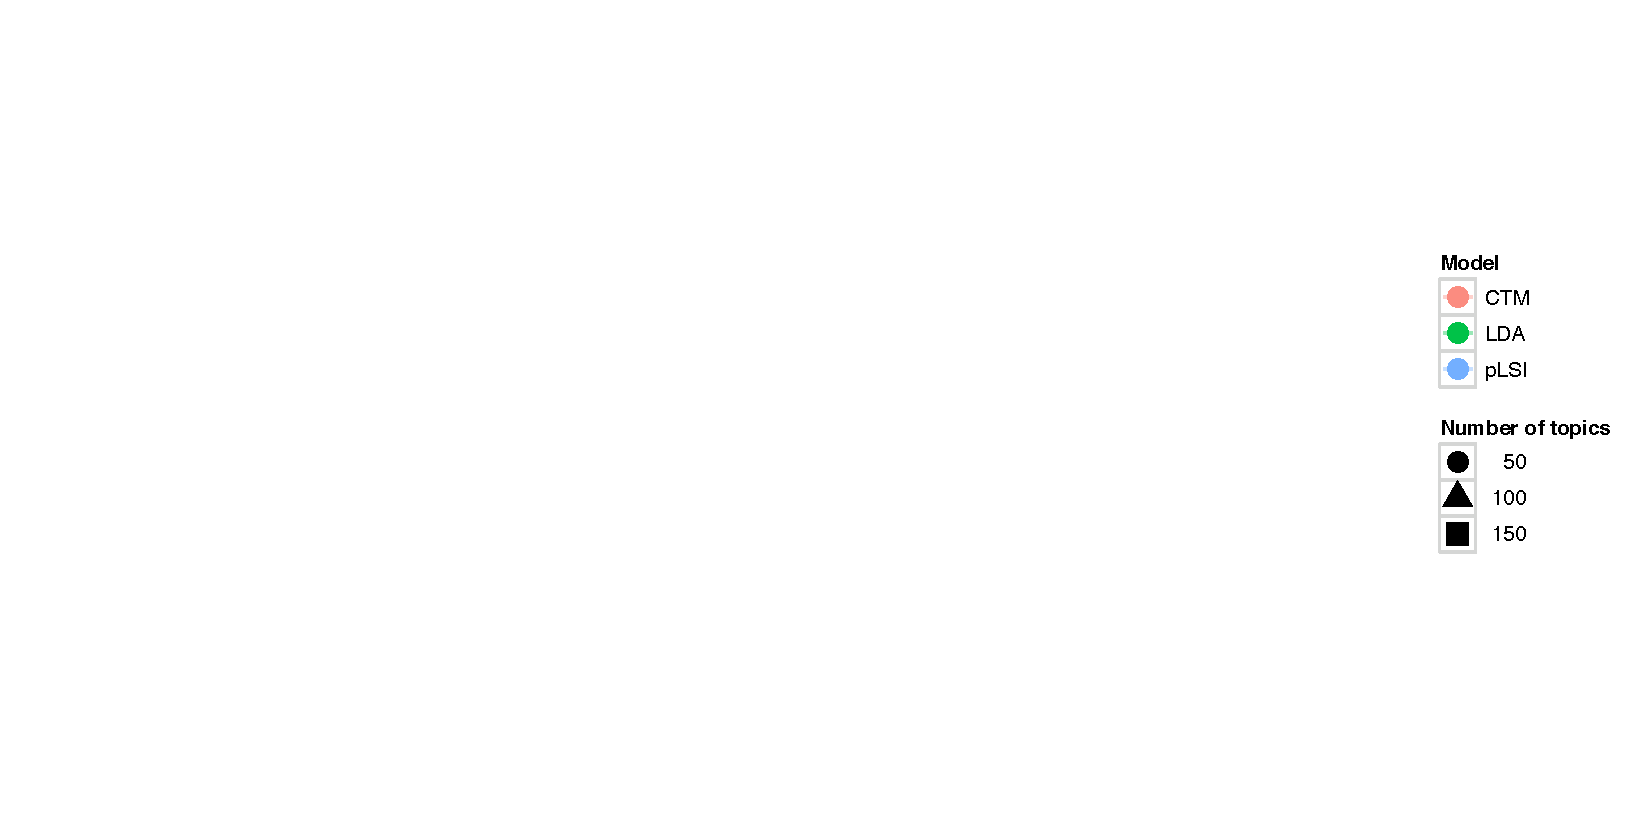
\includegraphics[scale=\graphscale]{reading_tea_leaves/tasks/legend}
\end{columns}
\vspace{-0.75cm}
\begin{center}
  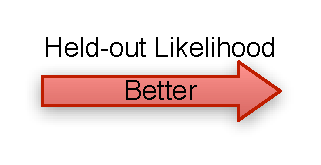
\includegraphics[scale=\graphscale]{reading_tea_leaves/tasks/held-out} \\
\only<1> {within a model, higher likelihood $\not =$ higher interpretability}
\only<2> {across models, higher likelihood $\not =$ higher interpretability}
\end{center}
}


\begin{frame}
  \frametitle{Evaluation Takeaway}

  \begin{itemize}
    \item Measure what you care about~\cite{chang-09c}
      \item If you care about prediction, likelihood is good
\item If you care about a particular task, measure that
    \end{itemize}

\end{frame}

\fi
